\chapter{Implementation and Testing}

\section{Translator}

\subsection{Recursive Expansion}
The main idea behind the Lispish compiler implementation is recursive expansion.
The compiler breaks down each s-expression it comes across into its primitives until there is no more work to be done. It then buils up the result in layers as the recursion folds upwards. 

\begin{figure}[hb]
	\centering
	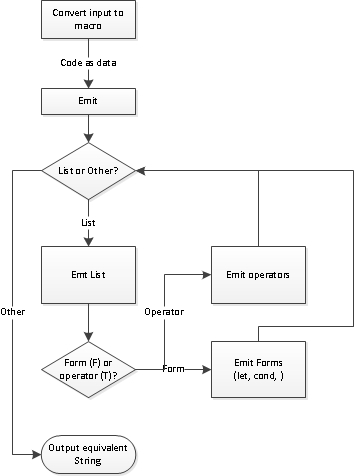
\includegraphics{Graphics/implementation_flowchart.jpg}
	\caption[Abstract \textit{Lispish to JavaScript} compilation.]
   {Abstract figure of \textit{Lispish to JavaScript} compilation.}
\end{figure}

Figure [NUMBER HERE] illustrates the functional flow chart of the compiler, without yet going deep into the details how s-expressions with multiply arity arguments are handled. 

\subsection{Forms with multiple arity (MapReduce)}

In order to solve the multiple arity problem, where for instance a (cond ) form can take multiple condition/true-form expression tuples and each one of them has to be individually compiled and them reduced to a string, a Map Reduce construct has been used. 

AARGGHH!!!

\section{Testing}
In order to ensure that the compiler is naturally expanded and a sufficient amount of regression tests is performed whenever a new language construct is added, I have decided to use the Test Driven Development methodology. 

\subsection{clojure.test API}
The tool to support me in the task of TDD I used was the clojure.test API.
clojure.test API [REFERENCE HERE] is a unit testing framework that provides a set of in-built forms, particularly the "is" macro that allows to perform boolean assertions on arbitrary expressions. 

\begin{quote}
\begin{verbatim}
(deftest factorial-example
  (is (= "function factorial(n) {if(n<2) { return 1 } else { return (n*factorial(((n-1)))) }}"
         (lisp-to-js (defn factorial [n] (if (< n 2) 1 (* n (factorial (- n 1)))))))))
\end{verbatim}
\end{quote}

.Although the compiler is not a very complexy system, it still 